\documentclass[fleqn]{article}
\usepackage{brochure-venturis}
\def\wLaTeX{L\kern-.25em\raisebox{.5ex}{\fontsize{70}{0}\selectfont
    \textsc{a}}\kern-.12em T\kern-0.1667em\raisebox{-.5ex}{E}\kern-.1em X}
\begin{document}
\noindent\begin{tabular}{
  @{}%	                   flush left margin
  b{.35\columnwidth}%	   logo
  @{\hspace{.03\columnwidth}}%        gap
  >{\huge\centering\color{DarkBlue}}p{.62\columnwidth}%	   headline
  @{}%                     flush right margin
}
  \raisebox{-55pt}{%
    \fontsize{80}{0}\selectfont\color{DarkGreen}
    hort}
&
     University of Victoria\linebreak
     Horticulture Club\par\vspace{8pt}\hrule height3pt
  \par\bigskip
  \fontsize{16}{18}\selectfont\itshape
  March 2023 Newsletter\linebreak
\end{tabular}

\noindent\begin{tabular}{@{}
                         p{.38\columnwidth}%		blurb
		         @{\hspace{.04\columnwidth}}% 	gap
		         p{.58\columnwidth}%		quotes
		         @{}%			implicit margin
}
\sffamily\lite\fontsize{16}{18}\selectfont\raggedright 
A tour of the greenhouse led by Dr. Patrick Von Aderkas, and\linebreak\
a social plant swap in the Student Union Building with lots of free propagules!
\par\medskip

\small\rightskip=0pt
\subsection*{\sffamily Featured Plant: Dendrophylax}
Dendrophylax is a genus of epiphytic neotropical orchids found throughout Mexico, Central America, The West Indies, and Florida. This genus is notable as, while seedlings may produce a low number of tiny leaves, the mature plants of many species have evolved to be leafless-instead possessing densely clustered photosynthetic roots that contain chlorophyll in addition to absorbing water and nutrients. One such species-Dendrophylax lindenii (the ghost orchid)-is found growing epiphytally on trees in swampy forests of southwest Florida, Cuba, and other Caribbean islands, and blooms a number of impressive pale white flowers between June and August.\quoted{Jacques, Discord (11/23/2022)}
\par\medskip
\par\bigskip

% Upcoming Events Box, uncomment when have things to add
%\begingroup
%  \setlength{\fboxsep}{3pt}\noindent
%  \fbox{\vbox to8pc{\hsize=.38\columnwidth
%    \advance\hsize by-2\fboxsep\advance\hsize by-2\fboxrule
%    \null\vfill\normalsize\centering
%    Upcoming Events
%    \par\medskip\footnotesize\tabcolsep1mm
%    \begin{itemize}[noitemsep]
%    \item Tomato Plant Sale: undetermined time/location.
%    \item More (Time / Location)
%    \item Upcoming (Time / Location)
%    \item Events (Time / Location)
%    \end{itemize}
%    \vfill}}
%\endgroup

\par\medskip
\begingroup
  \setlength{\fboxsep}{3pt}\noindent
  \fbox{\vbox to8pc{\hsize=.38\columnwidth
    \advance\hsize by-2\fboxsep\advance\hsize by-2\fboxrule
    \null\vfill\normalsize\centering
    Join the Club
    \par\medskip\footnotesize\tabcolsep1mm
    Any events are free to attend for everyone, including non-members.
    If you would like to stay up to date with events, we recommend checking this newsletter or joining the club Discord, where you can chat with other members.
    If you would like to join the list of members, contact us on Instagram: @uvichorticulture
    \vfill}}
\endgroup

\subsection*{\sffamily Featured Botanist : Gregor Mendel}
Gregor Mendel, an Austrian monk, is known as the father of modern genetics for his groundbreaking research on the heredity of traits in pea plants. He discovered the basic principles of inheritance, including dominant and recessive traits, which are still used by scientists today to study genetics in plants and animals. Mendel's work had a significant impact on botany, showing horticulturalists how they can selectively breed plants with desirable traits. Despite being largely ignored in his time, Mendel is now recognized as one whose contributions to botany and genetics continue to shape our understanding of the natural world.\quoted{Alex, Direct Submission (03/13/2023)}

&\large
% front RH blurb
\lettrine[lines=3]{H}{uffing} steam into the overcast March sky, tucked away from the rest of the science buildings on campus, lies a hidden gem: a greenhouse. This facility is used by students and staff of the Centre of Forest Biology and holds local and exotic plants used in undergraduate and graduate research. Dr. Patrick von Aderkas conducted a tour of the Bev Glover Greenhouse for members of the Horticulture Club on March 2nd, exhibiting some of the best plants the hothouse has to offer. \linebreak\

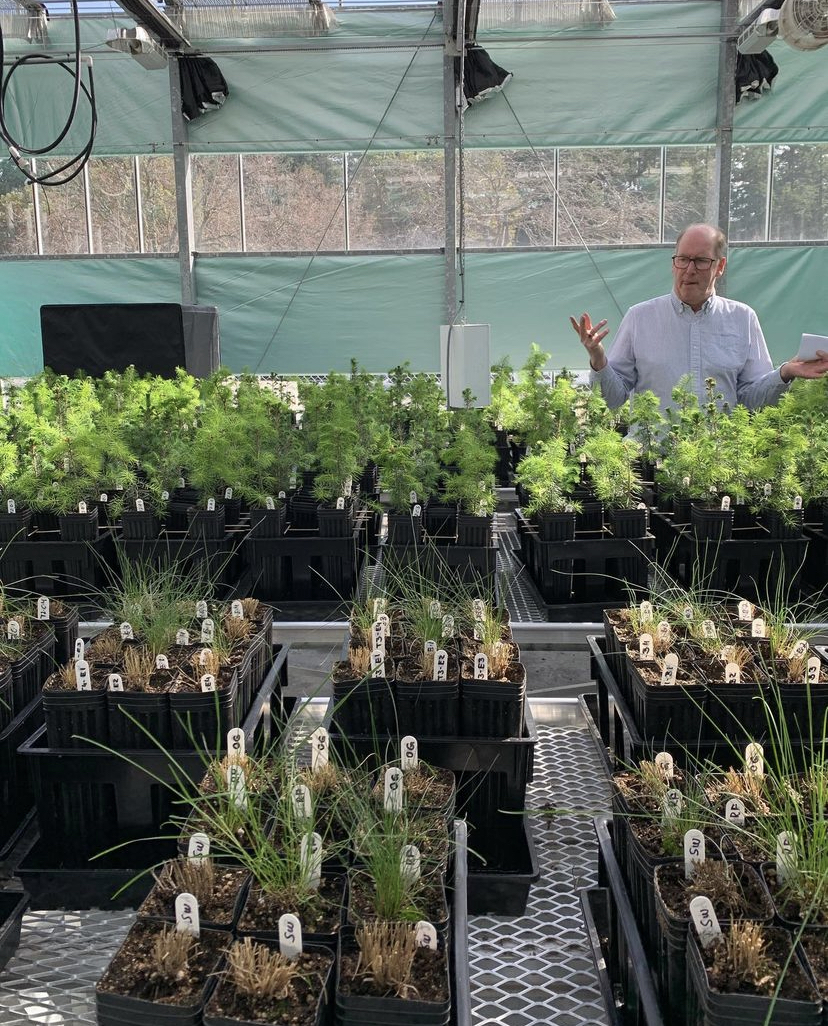
\includegraphics[width=.58\columnwidth]{greenhouse.jpg}

\bigskip
(Above: Dr. Patrick von Aderkas gave a tour of the Bev Glover Greenhouse on March 2nd.)

\end{tabular}

\clearpage
\end{document}
